\newpage 
\thispagestyle{empty}
\section{Design}
\subsection{Anforderungen}
Das Design des Antennensystems wird für einen Anwendungsfall im Freiraum dimensioniert. Die Distanz zwischen Sender und Empfänger soll 10 Meter betragen. Das Übertragungsmedium ist Luft, kann aber idealisiert als Vakuum angenommen werden. Das System soll isotrop abstrahlen und der Gewinn der Empfangsantenne kann mit einem Faktor  1 angenommen werden. Die Antenne soll symmetrisch gespiesen werden und im 2.4 GHz ISM Band arbeiten. Als Quelle dient ein Bluetooth Low Energie Texas Instruments CC2541 Chip mit 0 dBm als Sendeleistung. Als Designkriterien wird eine $S_{11}$ Dämpfung von -10 dB mit einer Bandbreite von midestens 100 MHz gefordert und eine Reserve von 6 dB soll in das Linkbudget eigerechte werden. Die Abbildung \ref{fig:DesignAusgangslage} zeigt die welsentlichen Punkte der Designanforderungen.

%%%%%%%%%%%%%%%%%%%%%%%%%%%%%%%%%
\begin{figure}[h]
\begin{center}
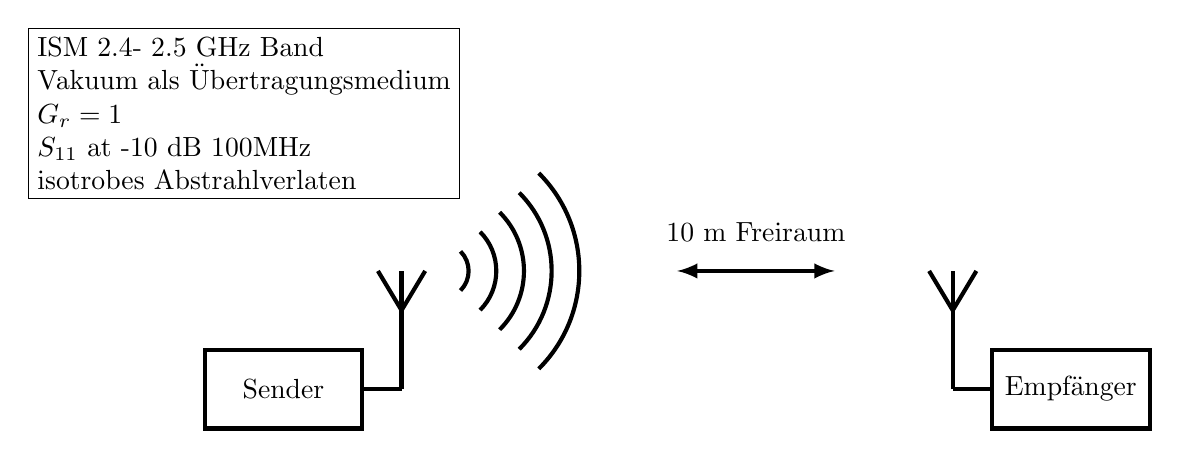
\begin{tikzpicture}
	\draw[line width=1.5pt](0, 0) rectangle (2, 1) node[pos=0.5] {Sender};
	\draw[line width=1.5pt] (2, 0.5) -- (2.5, 0.5);%zuleitung
	\draw[line width=1.5pt] (2.5, 0.5) -- (2.5, 1.5);%Antennenmast
	\draw[line width=1.5pt] (2.5, 1.5) -- (2.2, 2);%Antenne
	\draw[line width=1.5pt] (2.5, 1.5) -- (2.8, 2);
	\draw[line width=1.5pt] (2.5, 1.5) -- (2.5, 2);
	
	\draw[line width=1.5pt, <->, >=latex](6, 2)  -- (8, 2) node at (7, 2.5) {10 m Freiraum};
	
	\draw[line width=1.5pt] (9.5, 0.5) -- (10, 0.5);%zuleitung
	\draw[line width=1.5pt] (9.5, 0.5) -- (9.5, 1.5);%Antennenmast
	\draw[line width=1.5pt] (9.5, 1.5) -- (9.2, 2);%Antenne
	\draw[line width=1.5pt] (9.5, 1.5) -- (9.8, 2);
	\draw[line width=1.5pt] (9.5, 1.5) -- (9.5, 2);
	\draw[line width=1.5pt,decorate,decoration=expanding waves](3, 2) -- (5, 2);
	\draw[line width=1.5pt](10, 0) rectangle (12, 1) node[pos=0.5] {Empfänger};
	\node[draw,align=left] at (0.5,4) {ISM 2.4- 2.5 GHz Band\\ Vakuum als Übertragungsmedium\\ $G_{r} =1$\\ $S_{11}$ at -10 dB 100MHz \\ isotrobes Abstrahlverlaten};
\end{tikzpicture}
\end{center}
\caption{Design Ausgangslage}
\label{fig:DesignAusgangslage}
\end{figure}
%%%%%%%%%%%%%%%%%%%%%%%%%%%%%%%%%%%%%%%%%%

%\subsection{Technische Spezifikationen und Anforderungsliste}
%%\todo{Anforderungskatalogs mit Fest-, Mindest- \& Wunschforderungen}
%\begin{itemize}
%\item Geräte Connect 1
%\item Materialien des Gehäuse ABS Kusnstoff
%\item Volumen des Antennensystems
%\item Wirkungsradius 10m im Freiraum
%\item Richtcharakteristik isotroph
%\item Polarisation linear
%\item Antennen Wirkungsgrad ist zubestimmen
%\item Antennen Gewinn gleich wir der Abstrahl Wirkungsgrad
%\item minimaler Empfangspegel am Transceivers
%\item Transceivers Baustein Texas Instruments CC2541
%\item Sendeleistung
%\item $S_{11} \leq$ 10 dB
%\end{itemize}

\begin{table}[htb]
 \centering
\begin{tabular}{lccc}\toprule 
Nr. & Anforderung & Beschreibung & Wert   \\ 
001 & f & ISM Frequenzbereich  & 2.4-2.5 GHz  \\ 
002 & f & Handgerät lxbxh & 142x88x23 [mm]    \\  
003 & f &  Speisung des Antennensystems & symmetrisch  \\  
004 & f & Reflexionskoeffizient der Antenne  at -10B & 100 MHz  \\ 
005 & f & Funkdistanz, Arbeitsradius & 10m   \\ 
006 & f & Linkbudget Reserve & 6dB   \\ \bottomrule
  \end{tabular}
  \caption{Anforderungen an das Bluetooth Antennensystem}
  \label{AnforderungenAntenneSystem}
\end{table} 

\subsection{Design mit bekannten Modellen}

Die in der „Connect  1“ geforderte symmetrische Bluetooth Antenne soll   platzsparend im Inneren des Gerätes positioniert sein. Aus diesem Grunde wird eine gedruckte Dipolantenne entworfen. In kleinen  elektronischen Geräten sind auf eine Leiterplatte oder auf einem selbstklebenden Kunststoffstreifen gedruckte Antennen  von grossem Interesse. Die auf einer Leiterplatte oder einer Folie gedruckten Antennen haben den Vorteil, dass sie sehr kompakt und günstig zu produzieren sind. Zudem sind die Signalwege vom Sende- und Empfangschip zur Antenne sehr kurz. Trotz eines simplen Antennendesign haben Dipolantennen und Monopolantennen ein annähernd isotropes Abstrahlverhalten. Sie sind viel verbreitete Sende- und Empfangsantennen für tragbare Geräte. \\

Auf Grund ihrer simplen und kostengünstigen  Herstellung sind auf  einer Leiterplatte gedruckte Antennen sehr beliebt. Es entstehen nur geringe Kosten, weil die Antenne auf demselben PCB wie die gesamte Gerätelektronik gefertigt wird. Dies geschieht im selben Arbeitsgang der Print Fertigung. Die  Anpassung und die strahlenden  Antennenelemente sind ebenso Teil der Leiterplatte wie die Elektronikbauteil des Prints. Für ein System, bei dem ein isotropes Abstrahlverhalten gefordert ist, wie es in tragbaren Geräten oft der Fall ist, kommen oft Stabantennen zum Einsatz. 
Um eine gute Abstrahlleistung der Antenne zu erhalten, ist ein $\lambda /2$ Dipol ein guter Ansatz. Dabei erfordert es, dass die effektive mechanische Länge des Dipols etwas weniger als eine halbe Wellenlänge beträgt. Dies kann auf den Verkürtzungsfaktor zurückgeführt erden. Ein guter Ansatz ist 0.47 mal die Wellenlänge. 
Zur Berechnung der Länge des in Resonanz betriebenen Dipols kann die  Gleichung \ref{eq:lamba_2_laene_dipol} herangezogen werden.
\todo{Quelle}
\begin{equation}\label{eq:lamba_2_laene_dipol}
L=2l = 0.47 \lambda= 0,47 \dfrac{v}{f}
\end{equation} 
Wobei $v$ die tatsächliche Ausbreitungsgeschwindigkeit der Elektronen in den Dipol Radials ist. Diese Geschwindigkeit $v$ hängt von der effektiven dielektrischen Konstante der Umgebung der ab. 
Die effektive  Impulsgeschwindigkeit der Elektronen kann mit der Gleichung \ref{eff_Geschwindigkeit} berechnet werden. 
\begin{equation}\label{eff_Geschwindigkeit}
v = \dfrac{c}{\varepsilon_{eff}}
\end{equation}
Wobei $c$ die Lichtgeschwindigkeit im Vakuum und $\varepsilon_{eff}$  die effektive Dielektrizitätskonstante des umgebenden Mediums ist. Die effektive Dielektrizitätskonstante, einer auf ein Substrat gedruckte Antenne, ist von der  Geometrie und dem Dielektrikum des Substrats abhängig. Die Berechnung der effektiven Dielektrizitätszahl für eine schmale Kupferspur kann aus der Gleichung \ref{eff_epsilon} entnommen werden. 

\begin{equation}\label{eff_epsilon}
\varepsilon_{eff}=\dfrac{\varepsilon_r+1}{2}+\dfrac{\varepsilon_r-1}{2}\left[\left(1+\dfrac{12h}{w}\right)^{-\frac{1}{2}}+0.04\left(1-\dfrac{w}{h}\right)^{2}\right]
\end{equation}
Wobei $h$ die Dicke des Substrats, $w$ die Breite des Spuren und  $\varepsilon_{r}$ die relative Dielektrizitätskonstante des Substrats ist. 

\subsection{Design Ansatz $\lambda$/2 Dipolantenne}  
Unter Verwendung der in Kapitel \ref{sec:Implementierung} eingeführten Gleichungen \ref{eq:lamba_2_laene_dipol} soll eine Dipolantenne für die Frequenz 2.45 GHz entworfen werden. Die Antenne wird symmetrisch gespiesen. Die Antenne wird auf eine Leiterplatte gedruckt. Als Substrat des Antennenprints kommt eine Standard- FR-4 PCB mit einem geschätzten  $\varepsilon_r $ von 4.3 bei 1GHz und einer Substratdicke von 1,5 mm  zum Einsatz. Die Dicke der Kupferschicht beträgt 35 $\mu m$. Die Leiterbahnbreite für die Radials wird als 1mm breit definiert.\\

Wird die relative Dielektrizitätskonstante $\varepsilon_{r}$ in die Gleichung \ref{eff_epsilon} eingesetzt, so kann eine effektive Dielektrizitätszahl $\varepsilon_{eff}$  von xxxx berechnet werden.\\

Setzt man die effektive Dielektrizitätszahl $\varepsilon_{eff}$ von xxxxx  in die Gleichung der Elektronengeschwindigkeit aus der Formel \ref{eff_Geschwindigkeit} ein, so erhält man die Geschwindigkeit $v=vvv$. \\
Die Geschwindigkeit $v$  kann in der  Gleichung \ref{eq:lamba_2_laene_dipol} eingesetzt werden. Die Länge der Dipol Radials lässt sich bestimmen als:

\begin{equation}\label{eq:lamba_2_laene_dipol}
L=2l = 0.47 \lambda= 0,47 \dfrac{v}{f}=0,47 \dfrac{vvvv}{2.45[GHz]}=bla
\end{equation} 
\subsubsection{Simulatation einer Dipolantenne}
Es wurden vier Dipolantennen entworfen. Die Entwürfe sind im EMPIREXPU erstellt und simuliert worden. Die Antennenabmessungen wurden auf das Simulationsmodel optimiert. Die Länge der Antennen weicht vom $L=2l=\lambda/2$ Ansatz ab. Es wurde versucht eine optimale länge der Antenne für einen Einbau der Antenne in den "Connect 1" Geräten zu finden. Die Simulationen geht von einem 26$\mu$m dicken Kupfer als Antennenleiter aus. Dies enspricht dem 3M Kupferband des Typs "1181 Tape". Die Leimschicht des Klebeband wird vernachlässigt. Als Trägersubstrat dient direkt das ABS Gehäuse\cite{Kupferband}.
\subsubsection*{Entwurf}
Die vier Antennen habe alle dieselbe. Das "3M 1181 Tape" ist  hat eine Kupferstärke von 26$\mu$m. Die vier Antennen unterscheiden sich in der Breit der Kupferstreifen und in iher Form.\\
Es wurden die folgenden vier Formen simulieirt:
Dipol 5mm breit und xxmm lang
\begin{itemize}
\item Dipol 5mm breit und xxmm lang
\item Dipol 3mm breit und xxmm lang
\item Dipol 1mm breit und xxmm lang
\item Dipol 1mm breit und xxmm lang mit Dachkapazität
\end{itemize}

%%%%%%%%%%%%%%%%%%%%%%%%%%%%%%%%%
\begin{figure}[h]
\begin{center}
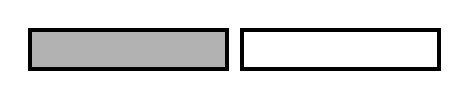
\begin{tikzpicture}
\draw[line width=1.5pt,fill=black!30](0, 0) rectangle (2.5, 0.5);
\draw[line width=1.5pt](2.7, 0) rectangle (5.2, 0.5);
\end{tikzpicture}
\end{center}
\caption{Dipol 5mm breit xxmm lang}
\label{fig:Dipol5mmxxlang}
\end{figure}
%%%%%%%%%%%%%%%%%%%%%%%%%%%%%%%%%

\begin{table}[h]
  \centering
  \begin{tabular}{l  c c c r} 
  \toprule 
  Antenne                  	& Freiraum/Conncect 1	&$S_{11}$	& $Z_{ant}$ 	& $\eta$\\ 
  \midrule
 5mm breit und xxmm lang    	& Freiraum				&			&  			&   		\\
            					& Conncect 1   			&      		&			&		\\
 3mm breit und xxmm lang    & Freiraum				&      		&			&		\\
     						& Conncect 1				&  			&			&		\\
 1mm breit und xxmm lang  	& Freiraum				&         	&			&		\\
      						& Conncect 1				&  			&			&		\\
  1mm breit und xxmm lang mit Dachkapazität  	& Freiraum				&         	&			&		\\
      						& Conncect 1				&  			&			&		\\
 \bottomrule
  \end{tabular}
  \caption{$\lambda/2$ Dipolantennen simuliert im Freiraum und im "Connect 1"}
  \label{tab:Vergeich_Lambda/2_Freiraum_Geraet}
\end{table}

\subsection{Neue Design Ansätze}